\section{CẤU HÌNH OSPF VÀ ECMP}\label{sec:ospf_ecmp}

Chương này trình bày chi tiết quá trình thiết kế sơ đồ mạng, cấu hình giao thức định tuyến động OSPFv3 và triển khai cơ chế cân bằng tải ECMP trên kiến trúc Leaf-Spine Pure IPv6 — hai kỹ thuật cốt lõi nhằm tối ưu hóa băng thông và khả năng chịu lỗi trên đường truyền trục chính (Backbone) của trung tâm dữ liệu.

\subsection{Thiết kế Topology Mạng}

\subsubsection{Mô hình Vật lý và Logic}

Hệ thống được thiết kế theo kiến trúc Leaf-Spine mở rộng, bao gồm tổng cộng 15 node mạng: 7 thiết bị định tuyến/chuyển mạch và 8 máy chủ đầu cuối. Sơ đồ tổng thể được minh họa trong Hình \ref{fig:topology}.

\begin{figure}[H]
    \centering
    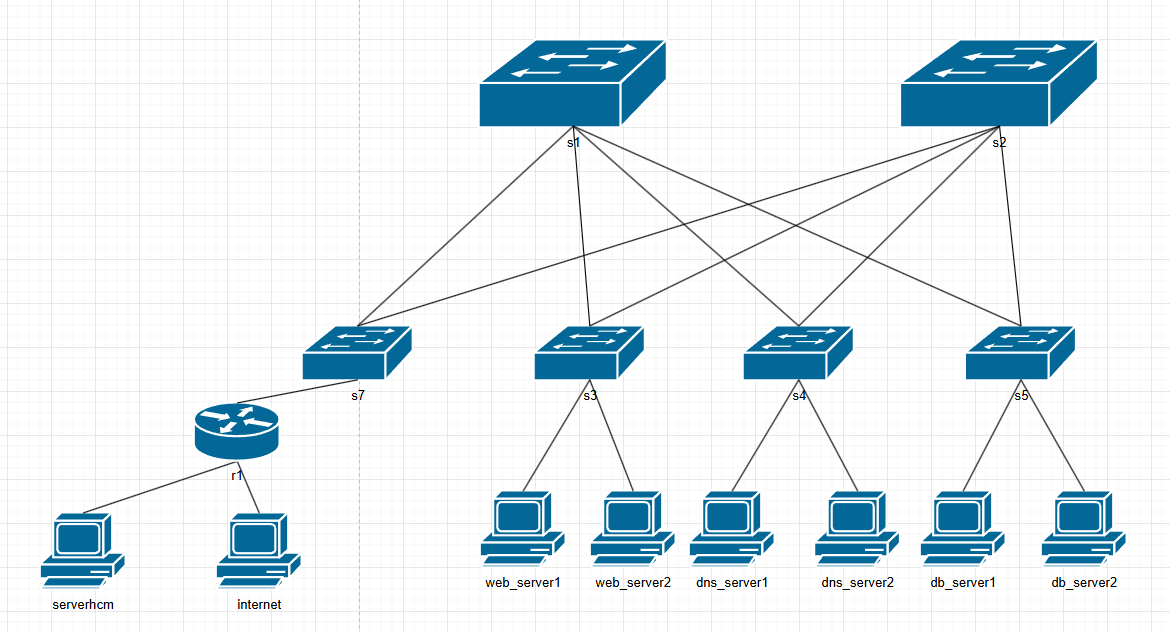
\includegraphics[width=\textwidth]{image/logic_network.png}
    \caption{Sơ đồ kiến trúc mạng Leaf-Spine Pure IPv6 với phân vùng chức năng.}
    \label{fig:topology}
\end{figure}

Vai trò cụ thể của từng lớp thiết bị:

\begin{table}[H]
    \centering
    \caption{Vai trò và chức năng của từng node trong hệ thống.}
    \label{tab:node_roles}
    \begin{tabular}{|l|l|p{8cm}|}
        \hline
        \textbf{Node} & \textbf{Vai trò} & \textbf{Chức năng} \\
        \hline
        S7 & Core Router & Kết nối trung tâm giữa Spine và Border Router. \\
        \hline
        S1, S2 & Spine (Lõi chia tải) & Chuyển tiếp lưu lượng East-West giữa các Leaf qua ECMP. \\
        \hline
        S3 & Leaf Web Tier & Kết nối web\_server1, web\_server2. Gateway fd00:10::254/64. \\
        \hline
        S4 & Leaf DNS Tier & Kết nối dns\_server1, dns\_server2. Gateway fd00:20::254/64. \\
        \hline
        S5 & Leaf DB Tier & Kết nối db\_server1, db\_server2. Gateway fd00:30::254/64. \\
        \hline
        R1 & Border Router & NAT64/Tayga, kết nối Internet IPv4. Redistribute default route. \\
        \hline
        internet & Host ngoại vi & Mô phỏng Internet (8.8.8.8/24). \\
        \hline
        serverhcm & Host ngoại vi & Mô phỏng máy chủ HCM (203.162.1.1/24). \\
        \hline
    \end{tabular}
\end{table}

\subsubsection{Sơ đồ Phân bổ Địa chỉ IPv6}

Toàn bộ mạng nội bộ hoạt động trên nền IPv6 thuần túy (Pure IPv6). Sơ đồ địa chỉ được thiết kế theo phân lớp chức năng, đảm bảo tính trực quan và dễ quản trị:

\begin{table}[H]
    \centering
    \caption{Sơ đồ phân bổ địa chỉ IPv6 trong hệ thống.}
    \label{tab:ipv6_scheme}
    \begin{tabular}{|l|l|p{6cm}|}
        \hline
        \textbf{Phân vùng} & \textbf{Dải địa chỉ} & \textbf{Mô tả} \\
        \hline
        Loopback Router & fc00:1111::X/128 & Router-ID duy nhất cho mỗi thiết bị \\
        \hline
        Core $\leftrightarrow$ Spine & fc00:3::0/126 & Liên kết P2P: S7-S1, S7-S2, S7-R1 \\
        \hline
        S1 $\leftrightarrow$ Leaf & fc00:1::0/126 & Liên kết P2P: S1-S3, S1-S4, S1-S5 \\
        \hline
        S2 $\leftrightarrow$ Leaf & fc00:2::0/126 & Liên kết P2P: S2-S3, S2-S4, S2-S5 \\
        \hline
        Web Subnet & fd00:10::/64 & web\_server1 (.1), web\_server2 (.2) \\
        \hline
        DNS Subnet & fd00:20::/64 & dns\_server1 (.1), dns\_server2 (.2) \\
        \hline
        DB Subnet & fd00:30::/64 & db\_server1 (.1), db\_server2 (.2) \\
        \hline
        VXLAN Overlay & fc00:100::/64 & Kênh truyền giữa các VTEP S3, S4, S5 \\
        \hline
    \end{tabular}
\end{table}

Lưu ý quan trọng: các liên kết Spine-Leaf sử dụng subnet \texttt{/126} (chỉ 4 địa chỉ, 2 khả dụng) — đây là best practice cho các liên kết Point-to-Point IPv6, tiết kiệm không gian địa chỉ và tăng tốc độ tra cứu bảng định tuyến.

\subsection{Triển khai Giao thức Định tuyến OSPFv3}

\subsubsection{Nền tảng FRRouting trên Mininet}

Mỗi thiết bị định tuyến trong hệ thống được triển khai dưới dạng lớp Python \texttt{FRRouter} kế thừa từ \texttt{Node} của Mininet. Khi khởi tạo, hệ thống tự động thực hiện chuỗi cấu hình Kernel bắt buộc:

\begin{lstlisting}[style=customcode, language=Python, caption={Lớp FRRouter — Cấu hình Kernel tự động cho định tuyến IPv6.}, label=lst:frrouter_class]
class FRRouter(Node):
    def config(self, **params):
        super(FRRouter, self).config(**params)
        # Bat IPv6 Forwarding
        self.cmd('sysctl -w net.ipv6.conf.all.forwarding=1')
        # Bat L4 Hash cho ECMP (cuc ky quan trong cho VXLAN)
        self.cmd('sysctl -w net.ipv6.fib_multipath_hash_policy=1')
        # Tat DAD de giam thoi gian khoi tao giao dien
        self.cmd('sysctl -w net.ipv6.conf.all.accept_dad=0')
        # Khoi chay Zebra (quan ly interface) va OSPF6D (dinh tuyen)
        self.cmd(f'/usr/lib/frr/zebra -d -f {confDir}/zebra.conf')
        self.cmd(f'/usr/lib/frr/ospf6d -d -f {confDir}/ospf6d.conf')
\end{lstlisting}

Tham số \texttt{net.ipv6.fib\_multipath\_hash\_policy=1} là yếu tố then chốt — nó kích hoạt thuật toán Hash L4 (băm dựa trên cổng TCP/UDP nguồn và đích) thay vì chỉ Hash L3 (IP), giúp phân tải hiệu quả hơn khi có nhiều luồng qua ECMP.

\subsubsection{Bơm Cấu hình OSPFv3 tự động qua VTY Console}

Cấu hình OSPFv3 được tự động hóa hoàn toàn bằng hàm \texttt{config\_ospf6\_via\_tcp()}, kết nối trực tiếp đến TCP port 2606 (VTY Console của daemon OSPF6D) và gõ lệnh theo cú pháp Cisco IOS:

\begin{lstlisting}[style=customcode, language=Python, caption={Hàm bơm cấu hình OSPFv3 tự động qua Netcat.}, label=lst:ospf_config]
def config_ospf6_via_tcp(node, rid, infts, r_extra=""):
    cmds = f"enable\nconf t\nrouter ospf6\nospf6 router-id {rid}\nexit\n"
    for i in infts:
        if i == 'lo' or i == 'br0':
            cmds += f"interface {i}\nipv6 ospf6 area 0\nexit\n"
        else:
            # Point-to-Point: loai bo bau cu DR/BDR, giam thoi gian hoi tu
            cmds += f"interface {i}\nipv6 ospf6 area 0\n"
            cmds += f"ipv6 ospf6 network point-to-point\nexit\n"
    if r_extra:
        cmds += f"router ospf6\n{r_extra}\nexit\n"
    cmds += "end\nwr\nexit\n"
    node.cmd(f'echo -e "{cmds}" | nc -w 1 127.0.0.1 2606')
\end{lstlisting}

Các liên kết Spine-Leaf được cấu hình kiểu \texttt{point-to-point} nhằm triệt tiêu quá trình bầu chọn Designated Router (DR) và Backup DR (BDR) — quá trình này thường tốn 40 giây và hoàn toàn không cần thiết trên các liên kết chỉ có 2 đầu.

\subsubsection{Cấu hình Đặc biệt cho Border Router R1}

Border Router R1 đóng vai trò đặc biệt: ngoài việc tham gia OSPFv3 Area 0, nó còn phải lan tỏa tuyến đường mặc định (\texttt{::/0}) xuống toàn bộ Spine-Leaf để các máy chủ nội bộ biết đường gửi gói tin NAT64 ra Internet:

\begin{lstlisting}[style=customcode, language=Python, caption={Cấu hình Redistribute và Default Route trên R1.}, label=lst:r1_config]
config_ospf6_via_tcp(r1, '100.100.100.100', ['r1-eth0', 'lo'], 
    "redistribute static\nredistribute kernel\n"
    "default-information originate always")
\end{lstlisting}

Tham số \texttt{default-information originate always} đảm bảo R1 luôn quảng bá tuyến mặc định ngay cả khi bản thân R1 chưa có default route trong bảng định tuyến, giải quyết vấn đề ``chicken-and-egg'' khi khởi tạo hệ thống.

\subsection{Tối ưu hóa Băng thông bằng Cơ chế ECMP}

\subsubsection{Nguyên lý Hoạt động của ECMP}

ECMP (Equal-Cost Multi-Path) là cơ chế cho phép router chuyển tiếp lưu lượng qua nhiều đường đi có cùng chi phí (metric) đến cùng một đích. Trong kiến trúc Leaf-Spine với 2 Spine, mọi cặp Leaf đều có chính xác \textbf{2 đường đi} với chi phí bằng nhau (qua S1 và qua S2):

\begin{itemize}
    \item \textbf{Tuyến 1:} Leaf S3 $\rightarrow$ Spine S1 $\rightarrow$ Leaf S5 (chi phí OSPF = 20)
    \item \textbf{Tuyến 2:} Leaf S3 $\rightarrow$ Spine S2 $\rightarrow$ Leaf S5 (chi phí OSPF = 20)
\end{itemize}

ECMP \textbf{không phải} là Round-Robin (chia đều từng gói). Thay vào đó, nó sử dụng \textbf{thuật toán băm (Hash)} đa trường để quyết định mỗi \textit{luồng} (flow) đi theo đường nào. Điều này đảm bảo tất cả các gói tin thuộc cùng một phiên TCP đi cùng một đường, tránh hiện tượng re-ordering gây giảm hiệu suất.

\subsubsection{So sánh Hash Policy L3 và L4}

\begin{table}[H]
    \centering
    \caption{So sánh hai chính sách Hash của ECMP.}
    \label{tab:hash_comparison}
    \begin{tabular}{|p{3cm}|p{5cm}|p{5cm}|}
        \hline
        \textbf{Tiêu chí} & \textbf{L3 Hash (Mặc định)} & \textbf{L4 Hash (Được bật)} \\
        \hline
        Trường Hash & IP nguồn + IP đích & IP + Port nguồn + Port đích \\
        \hline
        Entropy & Thấp (ít biến thể) & Cao (nhiều biến thể) \\
        \hline
        Phân tải & Kém (nhiều luồng cùng Hash) & Tốt (luồng phân tán đều) \\
        \hline
        VXLAN & Không hiệu quả (outer IP giống) & Hiệu quả cao (inner Port khác) \\
        \hline
        Cấu hình & Mặc định & \texttt{fib\_multipath\_hash\_policy=1} \\
        \hline
    \end{tabular}
\end{table}

Trong hệ thống thực nghiệm, L4 Hash được bật bắt buộc vì lưu lượng VXLAN có chung IP nguồn/đích (cặp VTEP), chỉ khác nhau ở cổng UDP nguồn ngẫu nhiên. Nếu chỉ dùng L3 Hash, toàn bộ VXLAN traffic sẽ đi qua một Spine duy nhất, vô hiệu hóa ECMP.

\subsubsection{Triển khai VXLAN Overlay L3VNI}

Để hỗ trợ giao tiếp liên phân vùng qua đường hầm ảo hóa, mỗi Leaf Switch được cấu hình làm VTEP (VXLAN Tunnel Endpoint):

\begin{lstlisting}[style=customcode, language=bash, caption={Cấu hình VXLAN VNI 100 và bảng FDB trên Leaf S3.}, label=lst:vxlan_config]
# Tao giao dien VXLAN voi VNI 100, port UDP 4789
ip -6 link add vxlan100 type vxlan id 100 dstport 4789 \
    local fc00:1111::3
ip link set vxlan100 up
ip -6 addr add fc00:100::3/64 dev vxlan100

# Bang FDB Unicast: chi dinh VTEP dich de tao Mesh
bridge fdb append 00:00:00:00:00:00 dev vxlan100 dst fc00:1111::4
bridge fdb append 00:00:00:00:00:00 dev vxlan100 dst fc00:1111::5

# Dinh tuyen uu tien qua VXLAN (metric 10 < OSPF metric 20)
ip -6 route add fd00:20::/64 via fc00:100::4 dev vxlan100 metric 10
ip -6 route add fd00:30::/64 via fc00:100::5 dev vxlan100 metric 10
\end{lstlisting}

Tuyến tĩnh với \texttt{metric 10} ưu tiên hơn OSPF (metric 20 mặc định), ép lưu lượng liên phân vùng nhất định phải đi qua đường hầm VXLAN. Gói tin VXLAN sau đó được lõi Spine chuyển tiếp qua ECMP — đây chính là điểm nút kết hợp giữa Overlay và Underlay.

\subsection{Tổng kết Chương}

Việc kết hợp OSPFv3 + ECMP + VXLAN trên kiến trúc Leaf-Spine tạo thành một hệ thống định tuyến thông minh ở nhiều tầng: OSPF tính toán đường đi tối ưu, ECMP phân tải qua nhiều Spine, và VXLAN cung cấp biệt lập phân vùng. Cấu hình hoàn toàn tự động thông qua kịch bản Python, giảm thời gian triển khai từ hàng giờ xuống dưới 1 phút cho toàn bộ 7 thiết bị.
